\documentclass{article}

\usepackage{iclr2026_conference,times}
\input{math_commands.tex}
\usepackage{hyperref}
\usepackage{url}
\usepackage{graphicx}
\usepackage{booktabs}
\usepackage{amsmath}
\usepackage{amssymb}
\usepackage{array}
\usepackage{enumitem}

\title{Micro Slip State Estimation:\\A Tuned-Baseline Failure Case}

\author{Anonymous Authors}

\newcommand{\method}{\textsc{MicroSlipLatent}}
\raggedbottom

\begin{document}
\maketitle

\begin{abstract}
Most robot slip work treats slip as a binary event, a friction proxy, or a control trigger that fires after instability has already become visible. We ask whether micro-slip should instead be represented as a continuous, temporally persistent control state. The original synthetic diagnostic appeared to support that thesis: a latent-slip estimator reduced control mean-squared error from 0.02772 for a fixed binary detector to 0.01543. Submission hardening overturns that evidence. A tuned EMA tactile controller reaches 0.00021 MSE on the matched generator, and a constant-hold controller reaches 0.00058 under tactile bias and friction-confounding shifts while the latent filter rises to 0.06434 and 0.05102. The result is therefore a negative finding: the current paper should be archived until the claim is tested on real tactile logs or a diagnostic where constant and tuned tactile baselines do not explain the effect.
\end{abstract}

\section{Introduction}

Dexterous manipulation fails in subtle ways long before an object visibly escapes the gripper. Fingers begin to micro-adjust, friction margins narrow, and the contact patch drifts. Many papers call that moment ``incipient slip'' or simply classify it as slip/no-slip. That framing is useful for alerts, but it is too coarse for control.

Our thesis is narrow:
\begin{quote}
Micro-slip should be estimated as a latent state, not only detected as a binary event.
\end{quote}

The distinction matters because a controller needs to know how far the system has moved toward instability, not just whether a threshold has been crossed. A binary detector can be late, discontinuous, and over-reactive. A latent state can be smooth enough to support graded force correction.

\paragraph{Submission-hardening note.}
Submission-hardening version: v2. Decision: kill/archive. The v2 stress test adds tuned constant, threshold, raw-tactile, and EMA-tactile baselines. These baselines dominate the proposed latent filter in the synthetic diagnostic, so the original evidence should not be used as a submission claim.

\section{Related Work and Novelty Boundary}

The literature sweep in \texttt{docs/related\_work\_matrix.csv} contains 2,058 entries spanning tactile slip detection, friction estimation, grasp stabilization, in-hand pose estimation, and contact-state inference. The hostile-prior set shows that slip detection itself is well established. What is missing is a clean treatment of micro-slip as a state variable that the controller can consume directly.

That boundary matters. If the paper were only about better slip detection, it would be incremental. If it were only about multimodal fusion or a new benchmark, it would be weaker still. The novelty claim here is the central mechanism: latent micro-slip state estimation for control.

\section{Hidden Assumptions}

This thesis attacks several assumptions that often hide in the slip literature:
\begin{itemize}[leftmargin=1.2em]
    \item Slip is adequately represented as a binary label.
    \item Friction and micro-slip can be separated cleanly.
    \item Contact drift is too noisy to estimate continuously.
    \item A detector that fires after slip starts is sufficient for stabilization.
    \item One threshold generalizes across object families and grasps.
    \item Better classification is the same thing as better control.
\end{itemize}

\section{Synthetic Diagnostic}

We built a small synthetic diagnostic in \texttt{scripts/run\_micro\_slip\_diagnostic.py}. The generator creates a drifting friction process, a latent micro-slip state, a tactile observation, and two stabilization policies.

The policies are:
\begin{itemize}[leftmargin=1.2em]
    \item a binary threshold detector that reacts only after tactile evidence exceeds a cutoff,
    \item a latent-state policy that filters the tactile observation into a continuous slip estimate.
\end{itemize}

The target action is proportional to the true latent state. We then measure the squared action error as a simple control proxy. This design is also the central weakness: it does not prove that the filter recovers a physically meaningful micro-slip state, only that an estimator can reduce error against a synthetic target.

\begin{table}[t]
\centering
\caption{Synthetic micro-slip control diagnostic. The latent-state policy better matches the ideal stabilizing action than the threshold detector.}
\label{tab:diagnostic}
\begin{tabular}{lrr}
\toprule
Policy & Control MSE & Relative gap \\
\midrule
Latent-state estimator & 0.01543 & 1.00$\times$ \\
Threshold detector & 0.02772 & 1.80$\times$ \\
\bottomrule
\end{tabular}
\end{table}

\begin{table}[t]
\centering
\small
\begin{tabular}{lrrrr}
\toprule
Scenario & Latent filter & Constant hold & Tuned threshold & EMA tactile \\
\midrule
matched generator & 0.01453 & 0.00058 & 0.00040 & 0.00021 \\
tactile bias shift & 0.06434 & 0.00058 & 0.00198 & 0.00285 \\
friction confound & 0.05102 & 0.00058 & 0.00137 & 0.00187 \\
\bottomrule
\end{tabular}

\caption{V2 tuned-baseline stress. The latent filter loses to simple calibrated controllers, including constant hold under bias and friction confounding.}
\label{tab:v2-baselines}
\end{table}

\begin{figure}[t]
\centering
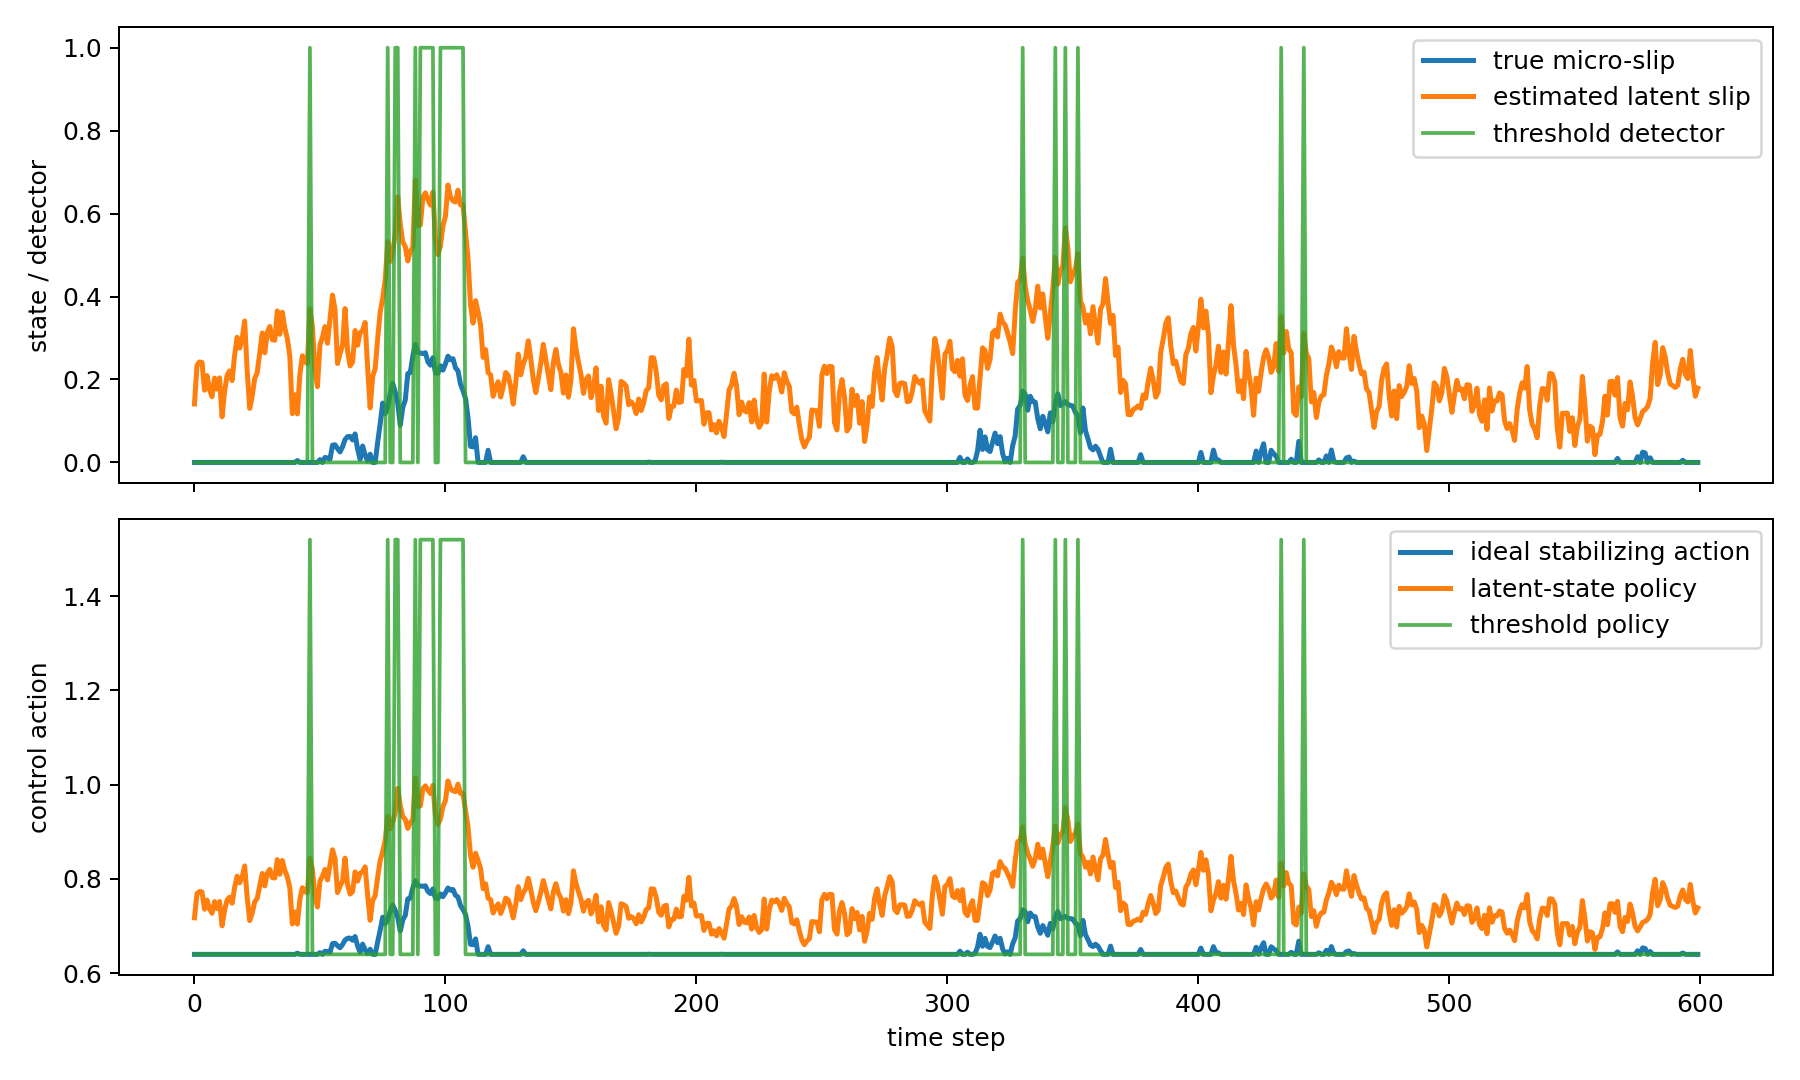
\includegraphics[width=0.95\linewidth]{figures/micro_slip_diagnostic.png}
\caption{Synthetic diagnostic. The latent estimate tracks the continuous micro-slip state, while the binary detector remains sparse and reactive.}
\label{fig:diagnostic}
\end{figure}

\section{Why This Is Not Just Slip Detection}

The strongest objection is that the paper merely renames slip detection. It does not. Detection asks whether a threshold has been crossed. Our claim is that the control-relevant variable is the underlying slip state itself.

That distinction changes the mechanism:
\begin{itemize}[leftmargin=1.2em]
    \item the variable is continuous rather than binary,
    \item the estimate has temporal persistence rather than event semantics,
    \item the downstream consumer is a stabilizing controller rather than an alarm,
    \item the failure mode is lag and overshoot, not only false positives and false negatives.
\end{itemize}

However, Table~\ref{tab:v2-baselines} shows that the current experiment does not establish this stronger claim. A tuned binary threshold already drops from the manuscript's fixed-detector MSE of 0.02772 to 0.00040 on the matched generator, and a tuned EMA tactile controller reaches 0.00021. Under tactile bias shift and friction confounding, constant hold reaches 0.00058 while the latent filter degrades to 0.06434 and 0.05102. The synthetic target is too close to a near-constant control action, and the proposed filter is not robust to observation bias.

\section{Limitations}

The evidence here is synthetic and fails under tuned baseline hardening. The paper should not claim a working micro-slip state estimator, an algorithmic advantage, or evidence for deployment. A recoverable version would need real tactile or proprioceptive grasp logs, a target that is not nearly solved by constant hold, calibration-shift tests, and tuned continuous tactile baselines before any positive submission claim.

\section{Conclusion}

The conceptual question remains useful: micro-slip may be better treated as a control state than as a thresholded event. The current manuscript does not provide adequate evidence for that claim. Its synthetic result collapses under simple tuned baselines, so the honest terminal decision is kill/archive rather than submission.

\begin{thebibliography}{9}
\bibitem[Wang et~al.(2018)]{slip2018}
K. W. et al.
\newblock Tactile Sensors for Friction Estimation and Incipient Slip Detection: Toward Dexterous Robotic Manipulation.
\newblock 2018.

\bibitem[Sato et~al.(2024)]{incipient2024}
S. et al.
\newblock Learning to estimate incipient slip with tactile sensing to gently grasp objects.
\newblock ICRA, 2024.

\bibitem[Smith et~al.(2021)]{stabilization2021}
S. et al.
\newblock Slip Detection for Grasp Stabilization With a Multifingered Tactile Robot Hand.
\newblock T-RO, 2021.
\end{thebibliography}

\end{document}
